\section{Alloy Model}
This section contains a possible formalization of the proposed system using the Alloy language.
The following alloy model is an attempt to represent the essential features of the system, in particular: the interactions between the users and the third parties for Data4Help and the generation and dispatch of an emergency notification for AutomatedSOS.
\par Due to the Alloy limitations, it was impossible to implement in the language the privacy condition that requires the presence of 1000 or more different users to accept a group data request. The limit was set to a symbolic value of 2 in the concerning predicate. \\

\lstinputlisting[language=alloy]{alloy/trackme.als}

\section{Proof of Consistency}
\begin{figure}[H]
    \renewcommand{\thefigure}{\alph{figure}}
    \makebox[\textwidth]{
        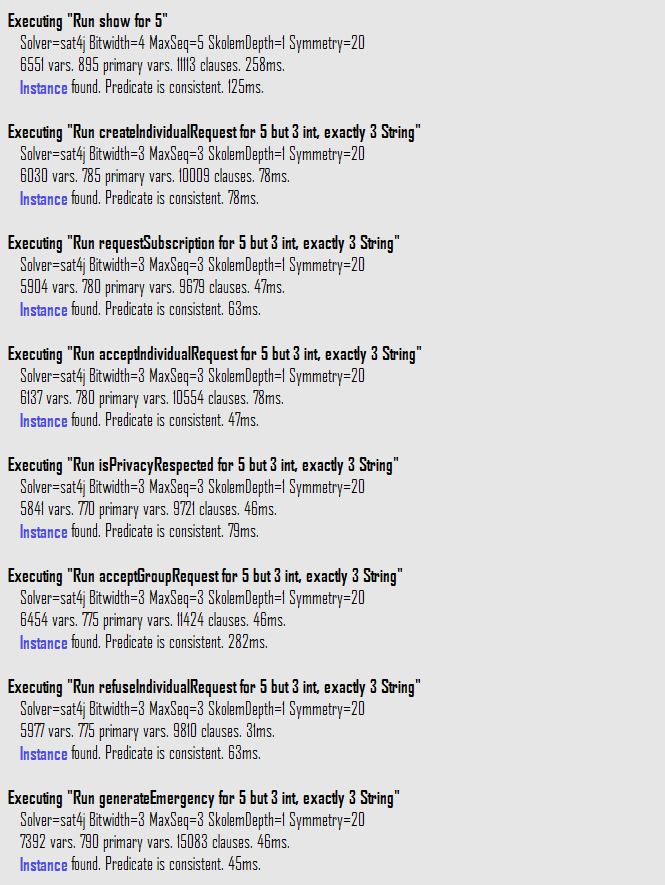
\includegraphics[width=1\linewidth]{alloy/alloy_result.png}
    }
    \captionsetup{labelformat=parens, labelsep=space, name=}
    \caption{Proof of Consistency}
\end{figure}


\section{Generated World}
\begin{figure}[H]
    \renewcommand{\thefigure}{\alph{figure}}
    \makebox[\textwidth]{
        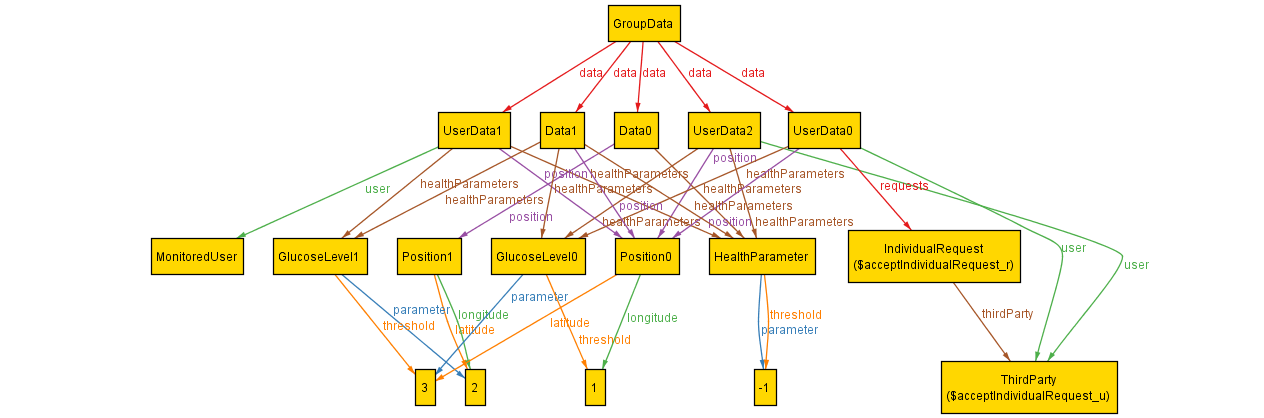
\includegraphics[width=1.55\linewidth]{alloy/alloy_world1.png}
    }
    \captionsetup{labelformat=parens, labelsep=space, name=}
    \caption{World 1}
\end{figure}

\begin{figure}[H]
    \renewcommand{\thefigure}{\alph{figure}}
    \makebox[\textwidth]{
        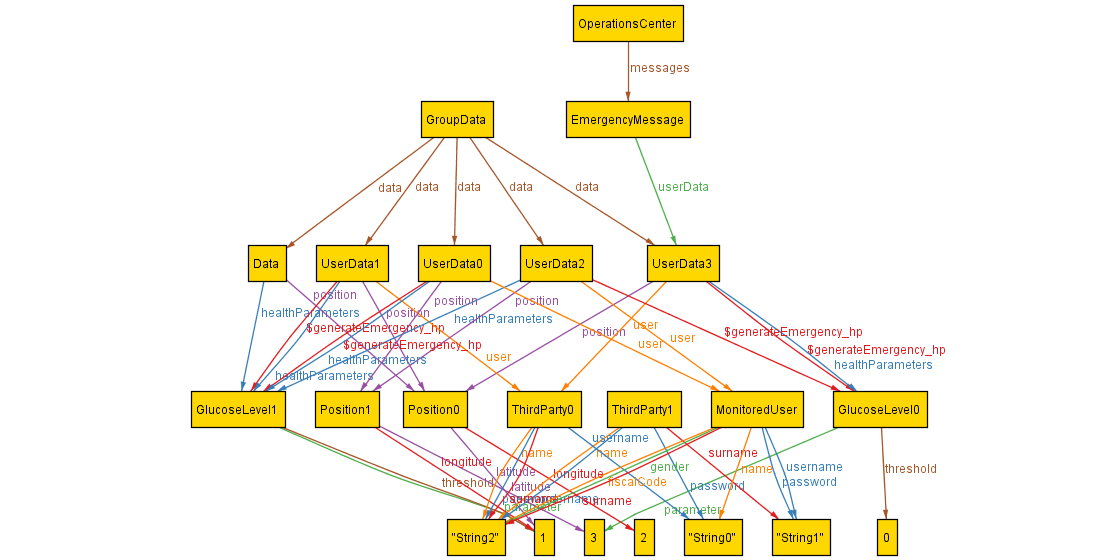
\includegraphics[width=1.55\linewidth]{alloy/alloy_world2.png}
    }
    \captionsetup{labelformat=parens, labelsep=space, name=}
    \caption{World 2}
\end{figure}